% Diagramas de bode

%%%%%%%%%%%%%%%%%%%%%%%%%%%%%%%%%%%%%%%%%%%%%%%%%%%%%%%%%%%%%%%%%%%%%%%%%%%%%%%%
% Exercício 1.
%%%%%%%%%%%%%%%%%%%%%%%%%%%%%%%%%%%%%%%%%%%%%%%%%%%%%%%%%%%%%%%%%%%%%%%%%%%%%%%%
\section*{Exercício 1}

\emph{Estude a estabilidade de Nyquist de:}

\begin{equation}
\label{equ:g1}
G(s) = \frac{K}{s^2(s+1)}; \qquad Z = P + N.
\end{equation}

\emph{Após determinar o intervalo, determine um K estável. A seguir, projete um controle avanço de fase:}

\begin{figure}[H]
    \centering
    \caption{\emph{Controlador em malha fechada.}}
    \includegraphics[scale=0.3]{ctrl}
    \label{fig:ctrl}
\end{figure}

\emph{com} $C(s) = K_c \left(\frac{s+Z_0}{s+P_0}\right)$ \emph{para} $mp \leq 5 \, \%$ \emph{e} $t_s \leq 1 \, s$.

\subsection*{Análise da estabilidade}

O sistema dado possui dois polos na origem, o que fará com que o diagrama de Nyquist possua dois círculos de raio infinito. O valor de K não interfere no deslocamento do gráfico, sendo assim, o sistema é instável para qualquer valor de K. O código \ref{cod:nyquist1} pode ser utilizado para verificar a variação no diagrama de Nyquist.

\lstinputlisting[caption={Código para gerar o diagrama de Nyquist, variando K, com o MATLAB.},label={cod:nyquist1}]{MATLAB/nyquist1.m}

\begin{figure}[H]
    \centering
    \caption{Diagrama de Nyquist para $ 1 \leq K \leq 10$.}
    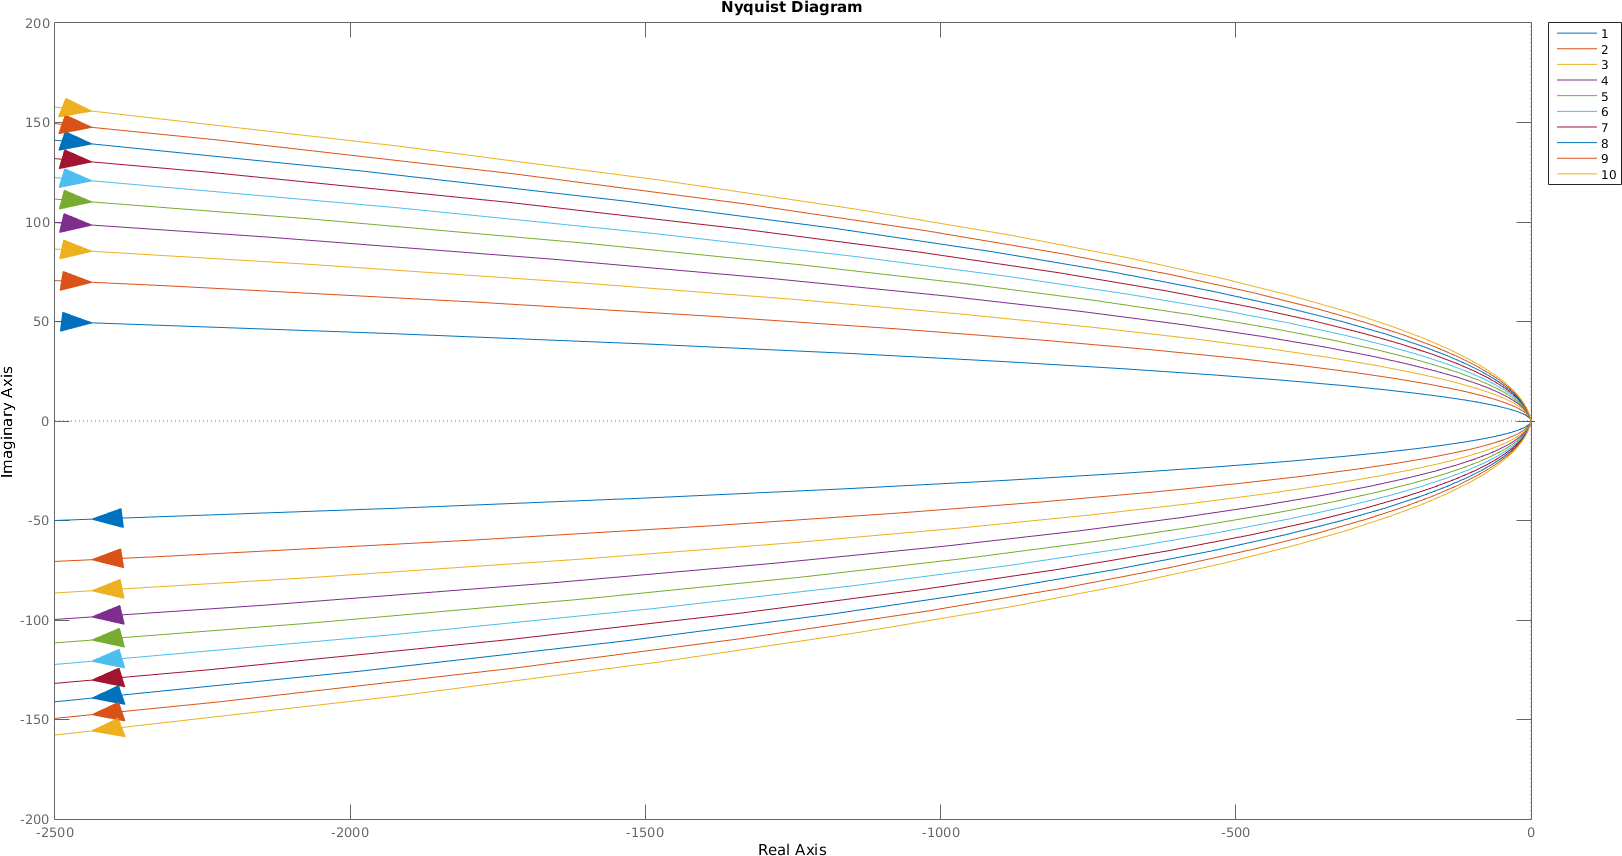
\includegraphics[scale=0.4]{nyquist1}
    \label{fig:nyquist1}
\end{figure}

Como pode ser observado na figura \ref{fig:nyquist1} (gerada a partir do código \ref{cod:nyquist1}), o valor de K não desloca o gráfico. Analisando a resposta ao degrau do sistema (figura \ref{fig:step1}), é possível observar o mesmo se mantem instável independente do valor de K.

\begin{figure}[H]
    \centering
    \caption{Resposta ao degrau para $ 1 \leq K \leq 10$.}
    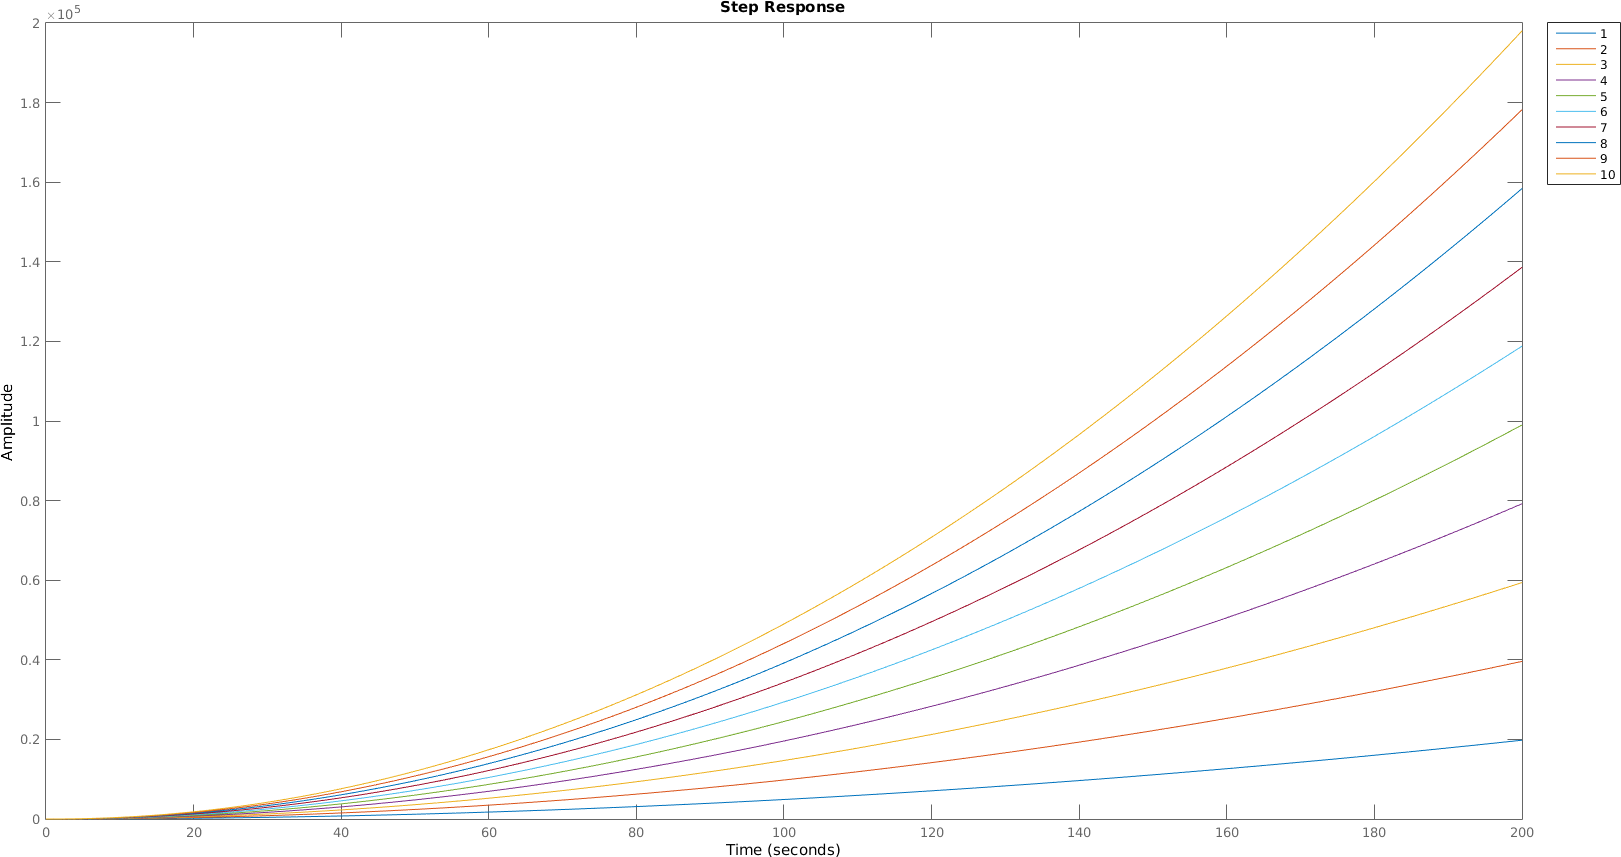
\includegraphics[scale=0.4]{step1}
    \label{fig:step1}
\end{figure}

\subsection*{Projeto do controlador}

Para $mp \leq 5 \, \%$, $\zeta \geq 0,7$ e para $t_s \leq 1 \, s$, $\omega_n \geq 4$ (aproximação de 2\%). Assim, os polos desejados são:

\[
    p = 6,3 \pm j6,3.
\]

O ângulo é:

\[
    \theta = tg^{-1} \left( \frac{6,3}{6,3} \right) \cong 45^\circ
\]

A contribuição angular do controlador é:
\[
    \beta = -180^\circ + 225^\circ = 45^\circ
\]

Devemos também adicionar um zero na origem, para poder utilizar o controlador de avanço de fase, assim, o controlador será:

\[
    C(s) = K_c s \left( \frac{s+4}{s+20} \right)
\]

O ganho $K_c$ foi determinado com o uso do recurso \emph{rctool} do matlab, sendo $K_c = 32.9$. A imagem \ref{fig:lead} mostra o \textit{root locus} do sistema, sendo que, a região em branco é a região que atende as especificações.

\begin{figure}[H]
    \centering
    \caption{\textit{Root Locus} para a planta $G(s)$ com o controlador $C(s)$.}
    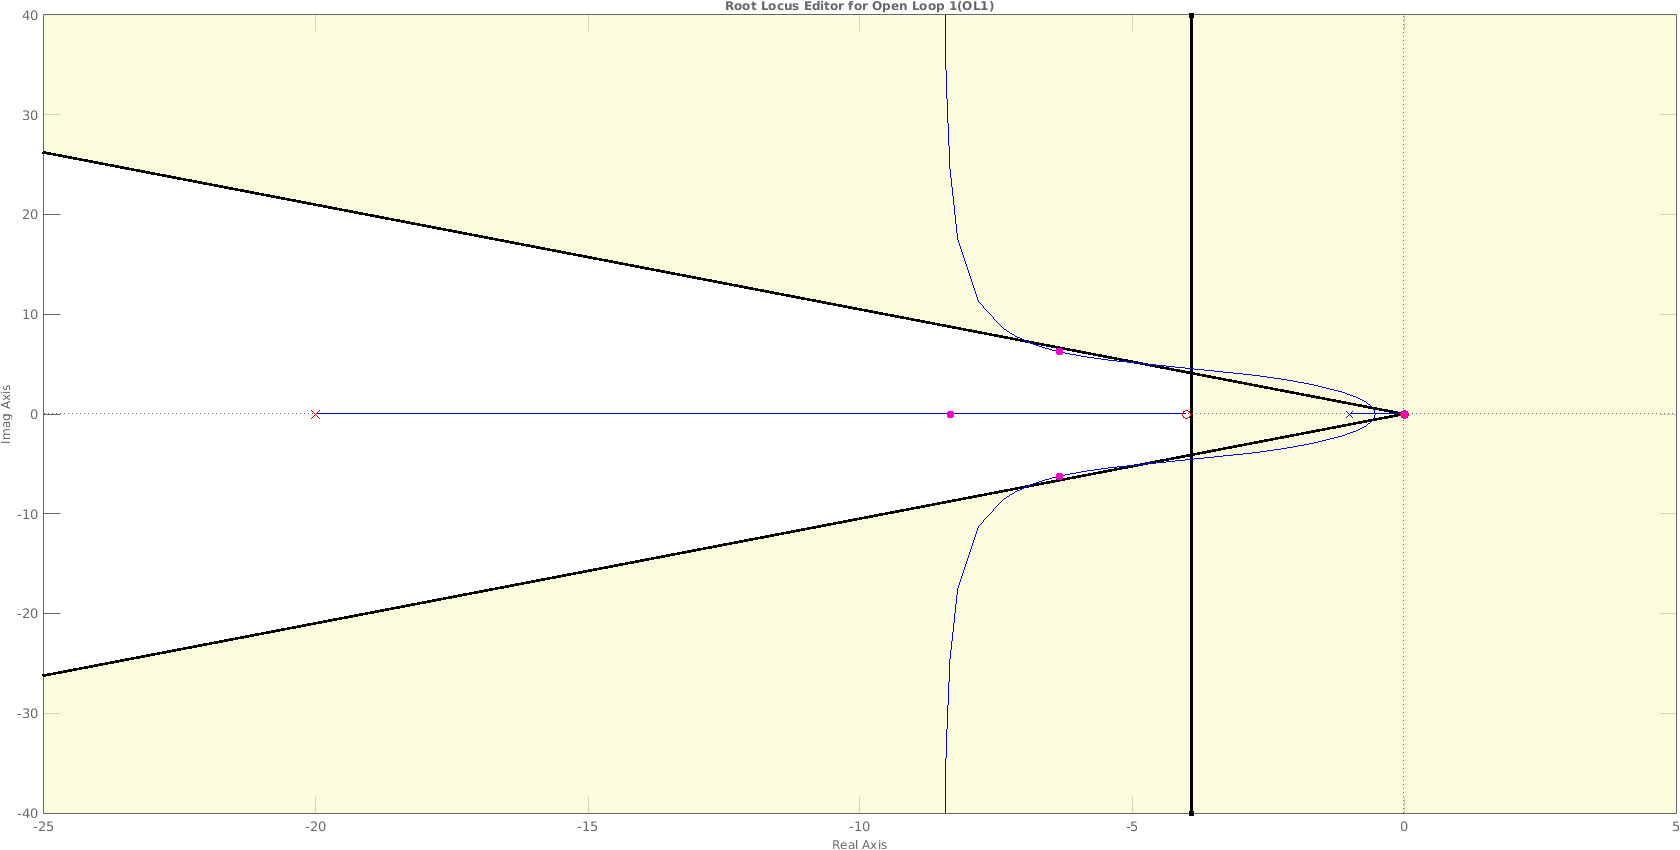
\includegraphics[scale=0.35]{lead}
    \label{fig:lead}
\end{figure}

\subsection*{Análise da estabilidade com o controlador}

Para confirmar a estabilidade do sistema, a figura \ref{fig:impulse} mostra que o sistema a resposta do sistema ao impulso unitário tende a zero e a figura \ref{fig:step2} mostra que o sistema é de fato estável para a entrada degrau.

\begin{figure}[H]
    \centering
    \caption{Resposta ao impulso do sistema.}
    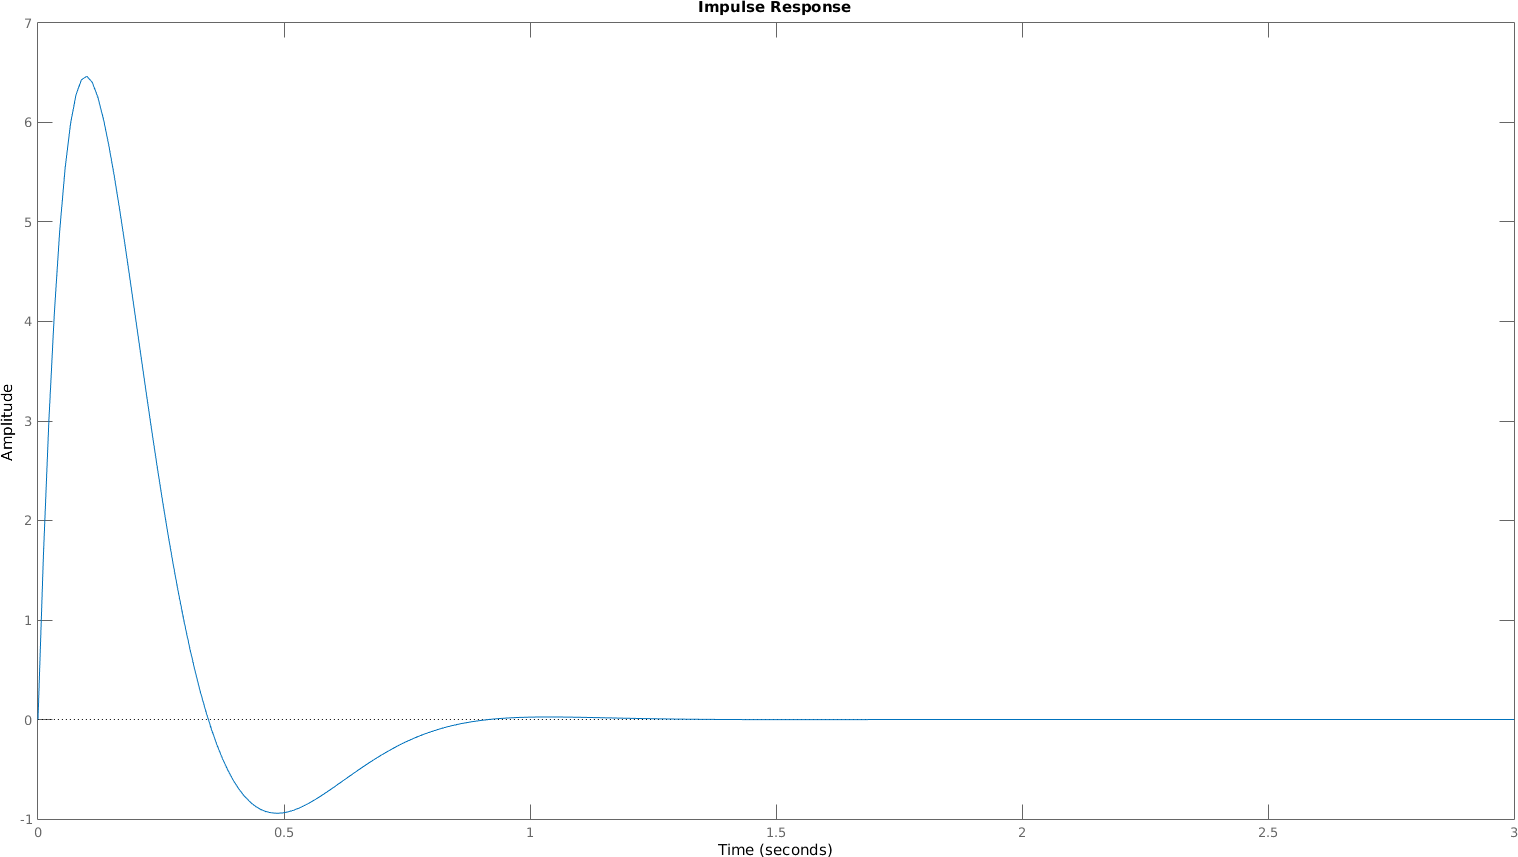
\includegraphics[scale=0.35]{impulse}
    \label{fig:impulse}
\end{figure}

\begin{figure}[H]
    \centering
    \caption{Resposta ao degrau do sistema.}
    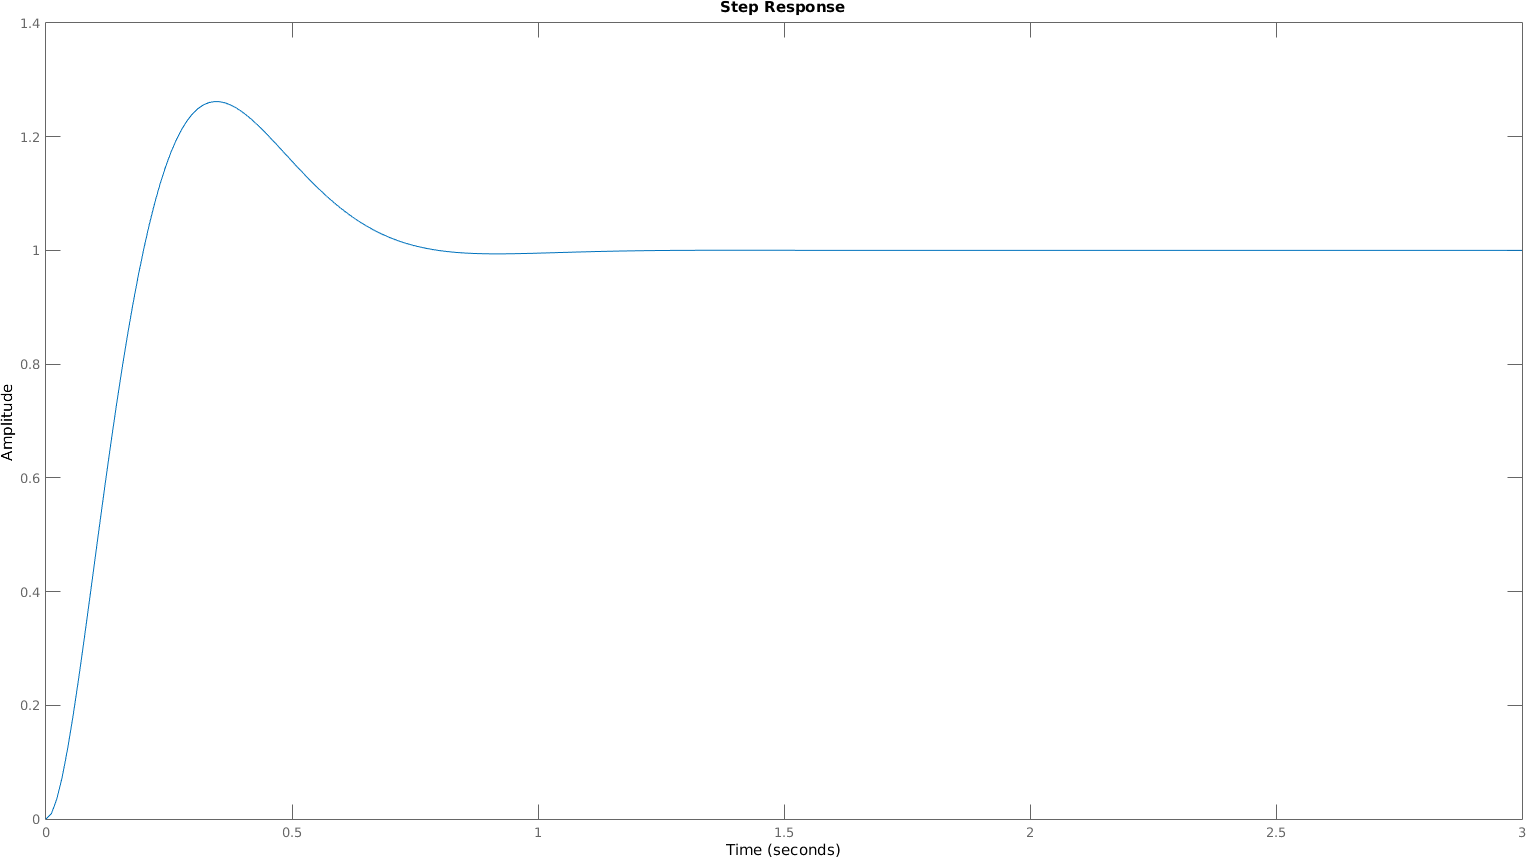
\includegraphics[scale=0.35]{step2}
    \label{fig:step2}
\end{figure}

Por ultimo, o diagrama de Nyquist, figura \ref{fig:nyquist2}, também mostra que o sistema é estável.

\begin{figure}[H]
    \centering
    \caption{Diagrama de Nyquist para o sistema.}
    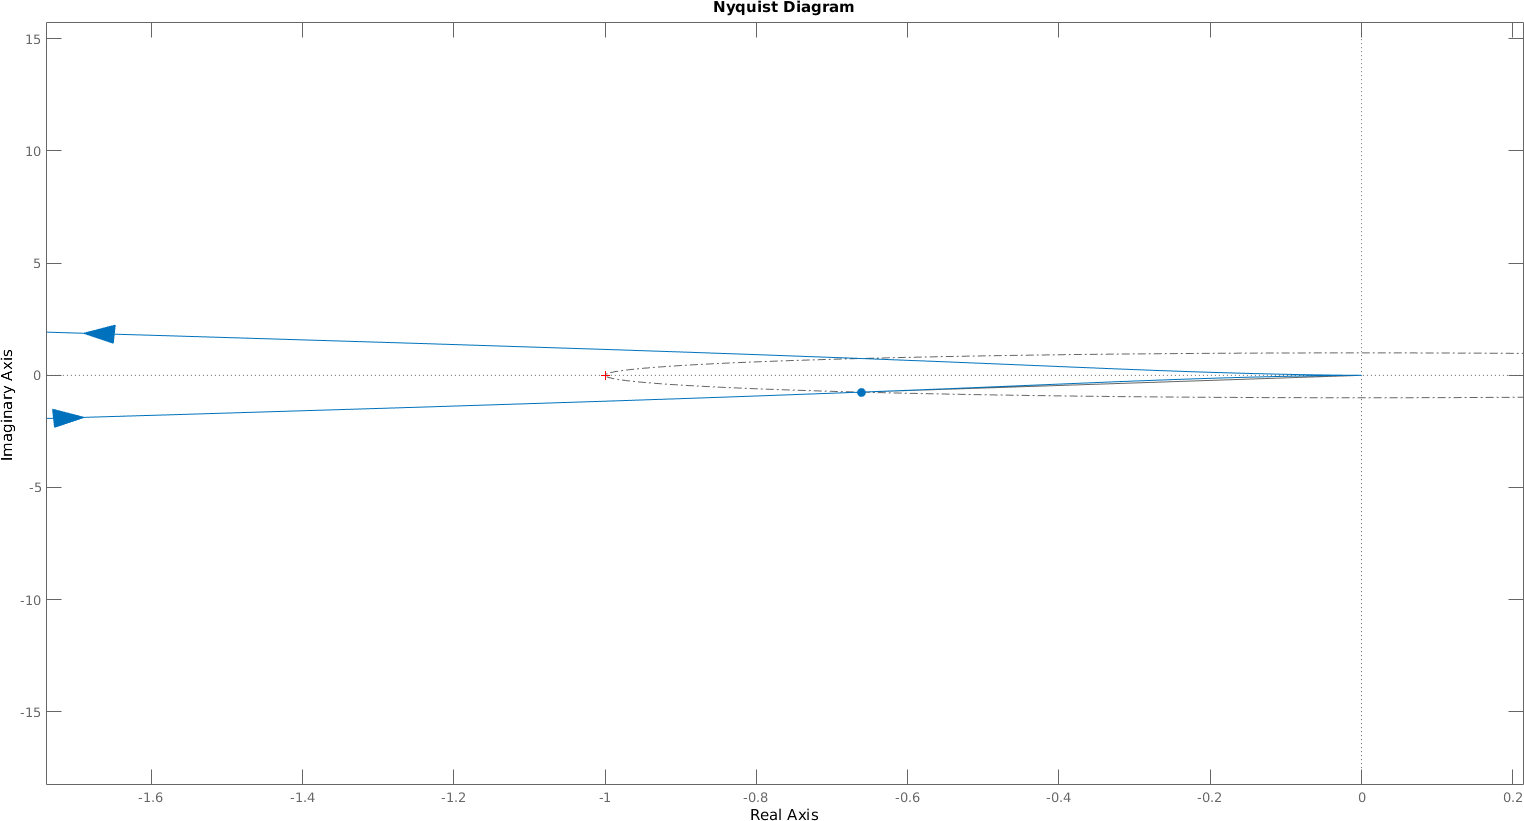
\includegraphics[scale=0.35]{nyquist2}
    \label{fig:nyquist2}
\end{figure}

